\documentclass[acmlarge]{acmart}
\AtBeginDocument{%
  \providecommand\BibTeX{{%
    \normalfont B\kern-0.5em{\scshape i\kern-0.25em b}\kern-0.8em\TeX}}}

\usepackage{geometry} % see geometry.pdf on how to lay out the page. There's lots.
\usepackage{amsthm}
\usepackage{url}
\geometry{a4paper} % or letter or a5paper or ... etc
% \geometry{landscape} % rotated page geometry
\theoremstyle{plain}
\newtheorem{thm}{Theorem}[section]
\newtheorem{lem}[thm]{Lemma}
\newtheorem{prop}[thm]{Proposition}
\newtheorem*{cor}{Corollary}

\theoremstyle{definition}
\newtheorem{defn}{Definition}[section]
\newtheorem{conj}{Conjecture}[section]
\newtheorem{exmp}{Example}[section]

\theoremstyle{remark}
\newtheorem*{rem}{Remark}
\newtheorem*{note}{Note}

% See the ``Article customise'' template for come common customisations

\title{Survey of ZK-SNARK}
\author{Yuncong Zhang}
\authornotemark[1]
\email{yczhangsjtu@163.com}
\affiliation{%
  \institution{Shanghai Jiao Tong University}
  \streetaddress{Dongchuan Rd. 800}
  \city{Minhang}
  \state{Shanghai}
  \postcode{200240}
}
% \date{} % delete this line to display the current date

%%% BEGIN DOCUMENT
\begin{document}

% \tableofcontents
% \newpage
\begin{abstract}
% ZK-SNARK (Zero-Knowledge Succinct Non-interactive ARgument of Knowledge) stands for the class of zero-knowledge schemes for NP statements that satisfy a series of requirements.
% As of this writing, there are a large number of zero-knowledge schemes that can be called ZK-SNARK.
% An important line of work, based on which Zerocash is implemented, is the pairing-based ZK-SNARKs originated from the work of Groth, etc.\ in 2010 and further made powerful by QAP proposed by Gennaro, etc.\ in 2013.
% Another line of work by Eli Ben-Sasson is based on short PCPs, and the state-of-art of which is called the ZK-STARK.
% Although STARK is not necessarily non-interactive, it can be made so easily via Fiat-Shamir heuristic.
% In this article, we will present a survey of the research that are related to ZK-SNARK.
\end{abstract}

\maketitle

\section{Introduction}

% The zkSNARKs are product of a series of studies~\cite{BlumFM88, SantisMP87, BabaiFLS91, Kilian92, Micali00, Groth06, GrothOS06Non, GrothOS06Perfect, Groth10, BitanskyCCT12} trying to improve \emph{zero-knowledge proofs} introduced by the ground-breaking work of Goldwasser, Micali, and Rackoff~\cite{GoldwasserMR85}.
% Zero-knowledge proofs allow a party to prove a statement to another party interactively without leaking secret information.
% As a variant, zkSNARKs additionally enjoy 1) non-interactivity, which allows formulating the proof in a string that can be transmitted and stored in places like blockchains; and 2) succinctness, which requires that the proof string is short and verification is sublinear to the statement size.
Zero-Knowledge Succinct Non-interactive ARgument of Knowledge (zkSNARK)~\cite{BitanskyCCT12} enables verifying computation outputs without knowing the inputs and faster than the original computation.
Currently, zkSNARKs are under active research, particularly due to their applications in blockchains~\cite{Ben-SassonCG0MTV14, SunALY17}, where zkSNARKs facilitate creating confidential transactions that conceal part or all of the transaction details.
Recent years have seen an explosion of zkSNARK implementations enjoying different properties including constant-size proofs~\cite{Groth16, GennaroGP013, Ben-SassonCGTV13, ParnoHG013, Ben-SassonCGTV13}, universal or trustless setups~\cite{GrothKMMM18, MallerBKM19, BunzFS20, Ben-SassonBHR18, Ben-SassonCRSVW19, AmesHIV17}, and post-quantum security~\cite{Ben-SassonBHR18, Ben-SassonCRSVW19}.


However, the rapid development of zkSNARK poses considerable challenges for researchers to keep up with the state-of-the-art.
Dozens of existing zkSNARK implementations rely on a large and increasing number of underlying tools of various efficiency, security, and functionalities.
It is also difficult to evaluate and compare existing schemes due to the high-dimensionality of measurement metrics including efficiency, security, and functionality.
Existing studies trying to overview this field are either oversimplifying~\cite{Nitulescu19, WalfishB15} or never tried to illustrate existing concrete implementations~\cite{ZKProof20}.
A comprehensive survey of literature in zkSNARKs can serve as an anchor of knowledge in this field of research, provide an overview of the most significant ideas behind current implementations, and inspire new perspectives to understand zkSNARKs.

% For example, a complete description of efficiency should at least consist of prover computation, verifier computation, proof size, and setup costs.
% The ZKProof Community recently initiated the standardization of zero-knowledge proofs and has presented a reference document~\cite{ZKProof20}.
% Despite being comprehensive, this document is more of an exhaustive reference of concepts than a systematic review of the literature.
% Other surveys including those by Nitulescu~\cite{Nitulescu19}, Walfish~\cite{WalfishB15} are also helpful for understanding the key concepts and research status of zkSNARKs.
% However, they each focus on a limited number of lines of progress.
% Nitulescu~\cite{Nitulescu19} describes the early history of zero-knowledge proofs and provides a detailed technical explanation of QAP/LIP-based implementations of zkSNARKs.
% Walfish~\cite{WalfishB15} illustrates the ideas behind implementations including Pinocchio~\cite{ParnoHG013}, Thaler~\cite{Thaler13}, Buffet~\cite{WahbySRBW15}, and TinyRAM~\cite{Ben-SassonCGTV13, Ben-SassonCTV14}.
% Both studies focus on the circuit-oriented designs and neglect those works that are more friendly with random access machines (RAMs)~\cite{Ben-SassonCGTV13, Ben-SassonCGV16, Ben-SassonBHR18}.



% \begin{table}[tb]
% 	\caption{Examples of zkSNARK building tools}
% 	\label{tab:build.tool}
% 	\centering
%
% 	\begin{tabular}{cccc}
% 	\hline
%
% 	\hline
% 	\textbf{Proof Model} & \textbf{Computation Model} & \textbf{Cryptography}\\
% 	\hline
% 		IP~\cite{GoldwasserMR85}       & Boolean circuit                  & Polynomial commitments~\cite{KateZG10} \\
% 		PCP/PCPP~\cite{BabaiFLS91}     & Arithmetic circuit               & CRH/ECRH \\
% 		IPCP                           & Structured circuit               & Bilinear pairing~\cite{BonehF01} \\
% 		IOP/IOPP~\cite{Ben-SassonCS16} & Layered circuit                  & Fiat-Shamir~\cite{FiatS86} \\
% 		LPCP/LIP~\cite{BitanskyCIPO13} & Random access machine            & Accumulator \\
% 		                               & QSP/QAP/SSP~\cite{GennaroGP013}  & Multi-party computation \\
% 		                               & AIR/ACSP~\cite{Ben-SassonBHR18}  & Lattic-based \\
% 		                               & R1CS                             & Group of unknown order~\cite{BunzFS20} \\
% 	\hline
%
% 	\hline
% 	\end{tabular}
% \end{table}

% \begin{table}[tb]
% 	\caption{Measurement metrics for zkSNARKs}
% 	\label{tab:measure}
% 	\centering
%
% 	\begin{tabular}{ccc}
% 	\hline
%
% 	\hline
% 	\textbf{Efficiency} & \textbf{Security} & \textbf{Functionality} \\
% 	\hline
% 		Prover complexity & Soundness & Expressiveness  \\
% 		Verifier complexity & Zero-knowledgeness & Public verifiability \\
% 		Setup complexity & Trusted setup & Universality \\
% 		Proof length & Post-quantum security & (Non)Preprocessing \\
% 		CRS length & Cryptographic assumption & \\
% 	\hline
%
% 	\hline
% 	\end{tabular}
% \end{table}

In this paper, we present a survey that overviews the current status of zkSNARKs.
First, we discuss the concepts that are necessary to understand the related literature.
Then we recall the history of zkSNARKs and examine the motivations and insights behind each major contribution.
Finally, we propose a framework for classifying and evaluating the zkSNARK implementations in terms of efficiency, functionality, expressiveness, infrastructure, building blocks, and security assumptions.
Using this framework, we reveal potential ways to leverage the existing underlying tools to construct new zkSNARKs with better combinations of properties.
We also point out promising directions in which we can design new useful tools.

% Zero-Knowledge Proof was first introduced by Goldwasser, Micali, and Rackoff in 1985 \cite{gmr1989knowledge}, which constructed a zero-knowledge proof for graph 3-colorability.
% Blum, Feldman and Micali followed their work and developed the concept of \emph{Non-Interactive Zero-Knowledge} (NIZK) proofs \cite{bfm1988non}, which eliminates the need of interaction by allowing the prover and the verifier to share a common reference string.
% However, their constructions of zero-knowledge schemes are not succinct.
% Then there came the PCP theorem \cite{bfls1991checking}, which basically says that for any NP language there exists a polynomial-size probabilistically checkable proof which is verifiable in polylogarithmic time.
% Based on the PCP theorem, Kilian \cite{kilian1992note} proposed the first construction of interactive zero-knowledge protocol in which the total amount of communication is less than the NP witness.
% After that, Micali \cite{micali2000computationally} proposed a succinct Non-Interactive Zero-Knowledge, by applying the Fiat-Shamir transformation on the work of Kilian.

% Above are the ground-breaking works for NIZKs.
% Almost all the subsequent works on NIZK directly or indirectly follow them.
% \section{Related Works}

% Following this work and the ground-breaking proposal of PCP by Babai et al.~\cite{BabaiFLS91}, Kilian~\cite{Kilian92} created the first \emph{succinct interactive argument} by compiling a PCP via cryptographic commitment, where the notation ``argument'' means the proof system has only computational soundness.
% After that, Micali~\cite{Micali00} constructed a succinct non-interactive argument by applying the Fiat-Shamir~\cite{FiatS86} transformation to Kilian's protocol.
% Since then, a decade of research has produced a large and ever-increasing number of zkSNARK implementations.

% \section{Preliminaries}
%
%   \subsection{Notations}
%
%    \paragraph{Elliptic curves.}
%
%   \subsection{Cryptographic Building Blocks}
%
%     \paragraph{Pairing.}
%
% \section{Interactive Proofs}
%
%   \subsection{Probabilistic Checkable Proofs}
%
% \section{Pairing-based ZK-SNARKs}
%
% The construction of ZK-SNARK in this line of work originates from a series of works by % Groth, Ostrovsky and Sahai \cite{groth2006simulation,gos2006non,gos2006perfect}, which % proposed constructions of NIZK based on bilinear groups.
% The state-of-the-art construction of ZK-SNARK is proposed by Groth in 2016 \cite{% groth2016size}, which will hereby be referred to as Groth16.
%
% \subsection{Quadratic Arithmetic Problems}
%
% \subsection{PCPs for QAP}
%
% \subsection{QAP-based NIZKs Without PCP}
%
% \section{PCP-based ZK-SNARKs}


% Fig.~\ref{fig:pp.zksnark} illustrates how preprocessing zkSNARK works.
% \begin{figure}[ht!]
% 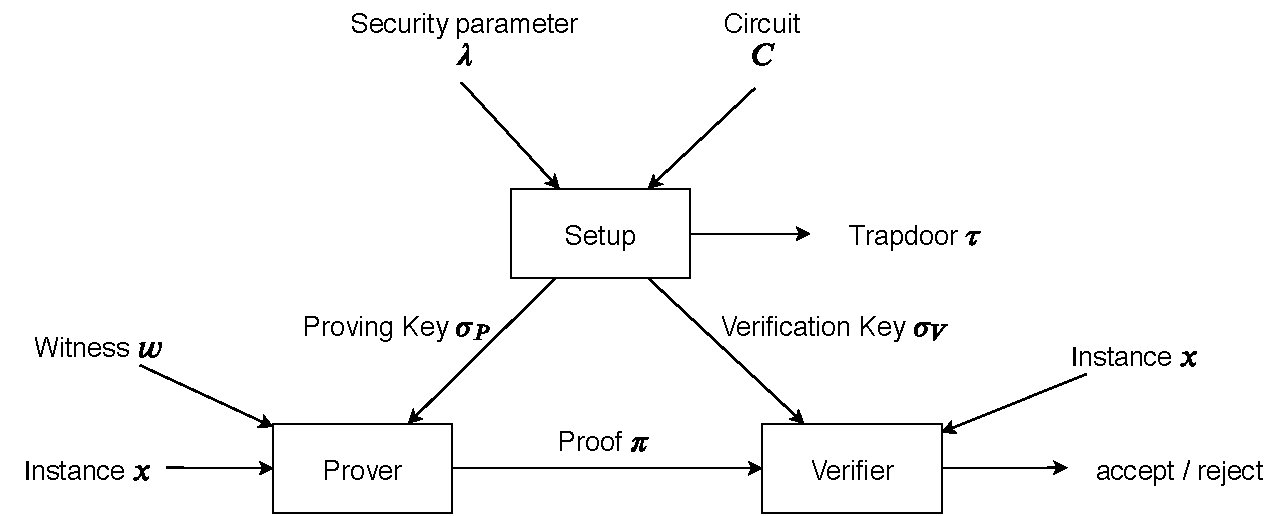
\includegraphics[width=0.4\textwidth]{images/ppzksnark.pdf}
% \caption{Preprocessing zkSNARK}
% \label{fig:pp.zksnark}
% \descriptionlabel{
% The $\Setup$ algorithm takes as inputs both the security parameter $\lambda$ and a circuit $C$, and outputs common reference strings, i.e. the proving key $\sigma_P$ and the verification key $\sigma_V$, to the prover and verifier respectively.
% $\Setup$ also outputs a trapdoor $\tau$ which enables simulating proofs without witness.
% The $\Prove$ algorithm takes as inputs an instance $x$ with corresponding witness $w$, together with proving key $\sigma_P$, and outputs the proof $\pi$ as validation of $x$.
% The $\Verify$ algorithm verifies the correctness of $x$ with proof $\pi$ and verification key $\sigma_V$, and decides if to accept or reject.}
% \Description{}
% \end{figure}


% In evaluating the efficiency of zkSNAKRs, the properties we care most about are proving time, verification time, proof sizes, and common reference string sizes.
% Fig.~\ref{fig:snark.sizes} summarizes the asymptotic complexities of current zkSNARK implementations.
% \begin{figure}[ht!]
% 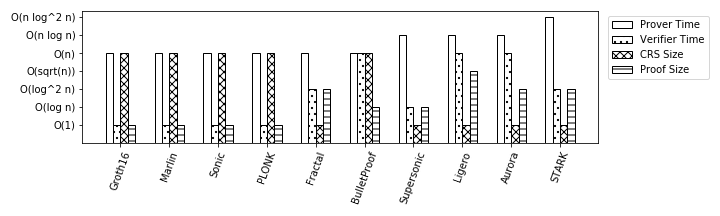
\includegraphics[width=0.5\textwidth]{images/complexity.png}
% \caption{Asymptotic complexities of zkSNARK implementations}
% \label{fig:snark.sizes}
% \descriptionlabel{
% The big-$O$ notation here hides the security parameter $\lambda$.
% The $n$ denotes the statement size.
% For circuit-based zkSNARKs, $n$ is the circuit size.
% For statements with succinct representation, e.g. STARK, $n$ is the length of execution trace, i.e. the size of the circuit representing the unrolled computation.}
% \Description{}
% \end{figure}

\bibliographystyle{alpha}
\bibliography{reference}

\end{document}